
\chapter{Linear Models}
\section{Model assumptions}
Assumptions (when correct) are a great tool to improve an algorithm. They can however lead to overfitting. For K-NN the only assumption that's made is the fact that proximity relates to label. 

\begin{definition}[Bias]
	The bias of a model is how strong its assumptions are.
\end{definition}

K-NN and Decision Trees are considered to be low bias. 

\section{Linear models}
A high-bias assumption is linear separability, which means that the classes can be simply divided by a line (or hyperplane in n dimensions).

A line is defined by a pair of values: 

\[
0 = w_1f_1 + w_2f_2
\]

To classify we can input the values into the equation. If it's positive it will be above the line and viceversa.

In n-dimensions: 

\[
0 = b+ \sum_{i=1}^{n} w_if_i
\]

\section{Online learning}

This linear model is different because it sees one example at a time. This is useful when taking in data streams (for example from online resources).

The algorithm receives an unlabeled example, it predicts and if it is not correct it updates its model.

\section{Perceptron algorithm}
This is a linear model that constantly updates when not correct.

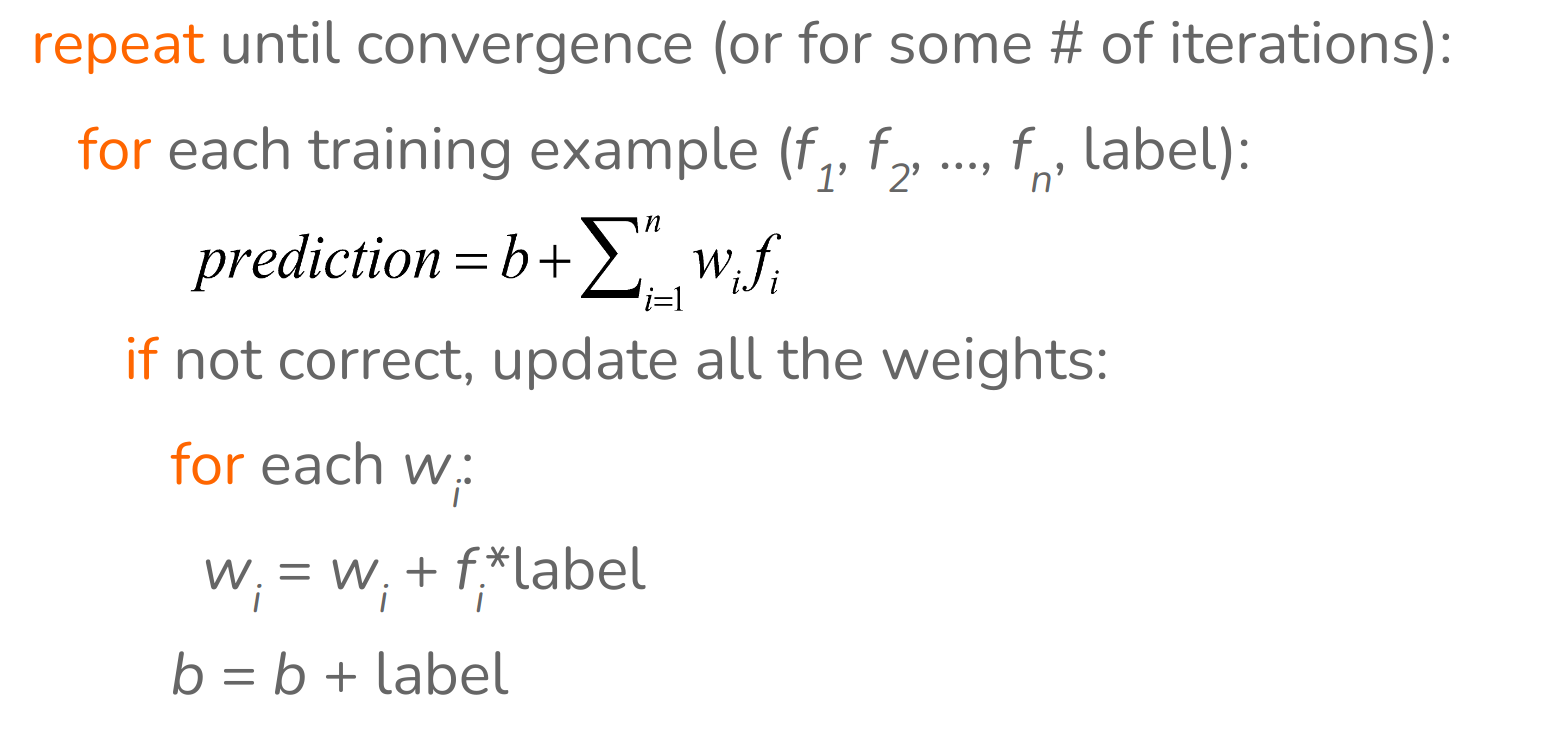
\includegraphics[scale=0.25]{perceptron}